Wireless Sensor Network (WSN) is a set of tiny distributed wireless nodes that have to collaborate and cooperate on a common distributed application to perform tasks specified by a user (Fig.~\ref{fig:scenario}). Recently, the development of WSNs has received an increasing interest due to the fast technological advances in the fields of sensor technology, low power microelectronics, and low energy wireless communications.
These networks are currently used in wide range of applications in the scientific, medical, commercial, and military domains, like for instance home automation, environment monitoring, industrial control, surveillance, security, healthcare, etc. 

In this context, WSNs are intimately tied to and inherently dependent on an environment they operate in. It leads to a necessity to adapt to an unpredicted environmental dynamics. Adaptation at run-time provides more flexibility in such software behavior as energy management, network protocols, architecture reconfiguration and error handling.
In fact, the application of self-organization concept to wireless sensor networks is seen as a key driver for improving the operation and maintenance of these networks. Thus, the self-organization can help reducing the cost of installation and management by simplifying some operational tasks through automated mechanisms pointing the self-configuration, self-optimization and self-healing~\cite{son_marchetti}.
Regarding self-configuration, it is triggered by incidental events for instance to add a new site or to introduce a new service or a new network feature. In that case, these lasts can require a re-configuration of a number of radio parameters or several resource management algorithms.
For the self-optimization in WSNs, intelligent methods are applied to the processed measurements to derive an updated set of the radio parameters or the resource management parameters~\cite{son_marchetti}.
Sensor nodes and wireless links are subject to different errors in function of the size of perturbation in time, space, and energy. So applying self-healing methods can resolve these problems and the loss of coverage or capacity induced by such events~\cite{son_marchetti}.
In this regard, WSNs increasingly need self-organization, self-configuration and self-adaptation to changing conditions to ease management and operation~\cite{son_sengul}.


\begin{figure}[t]
\vspace{-4mm}
\centering
 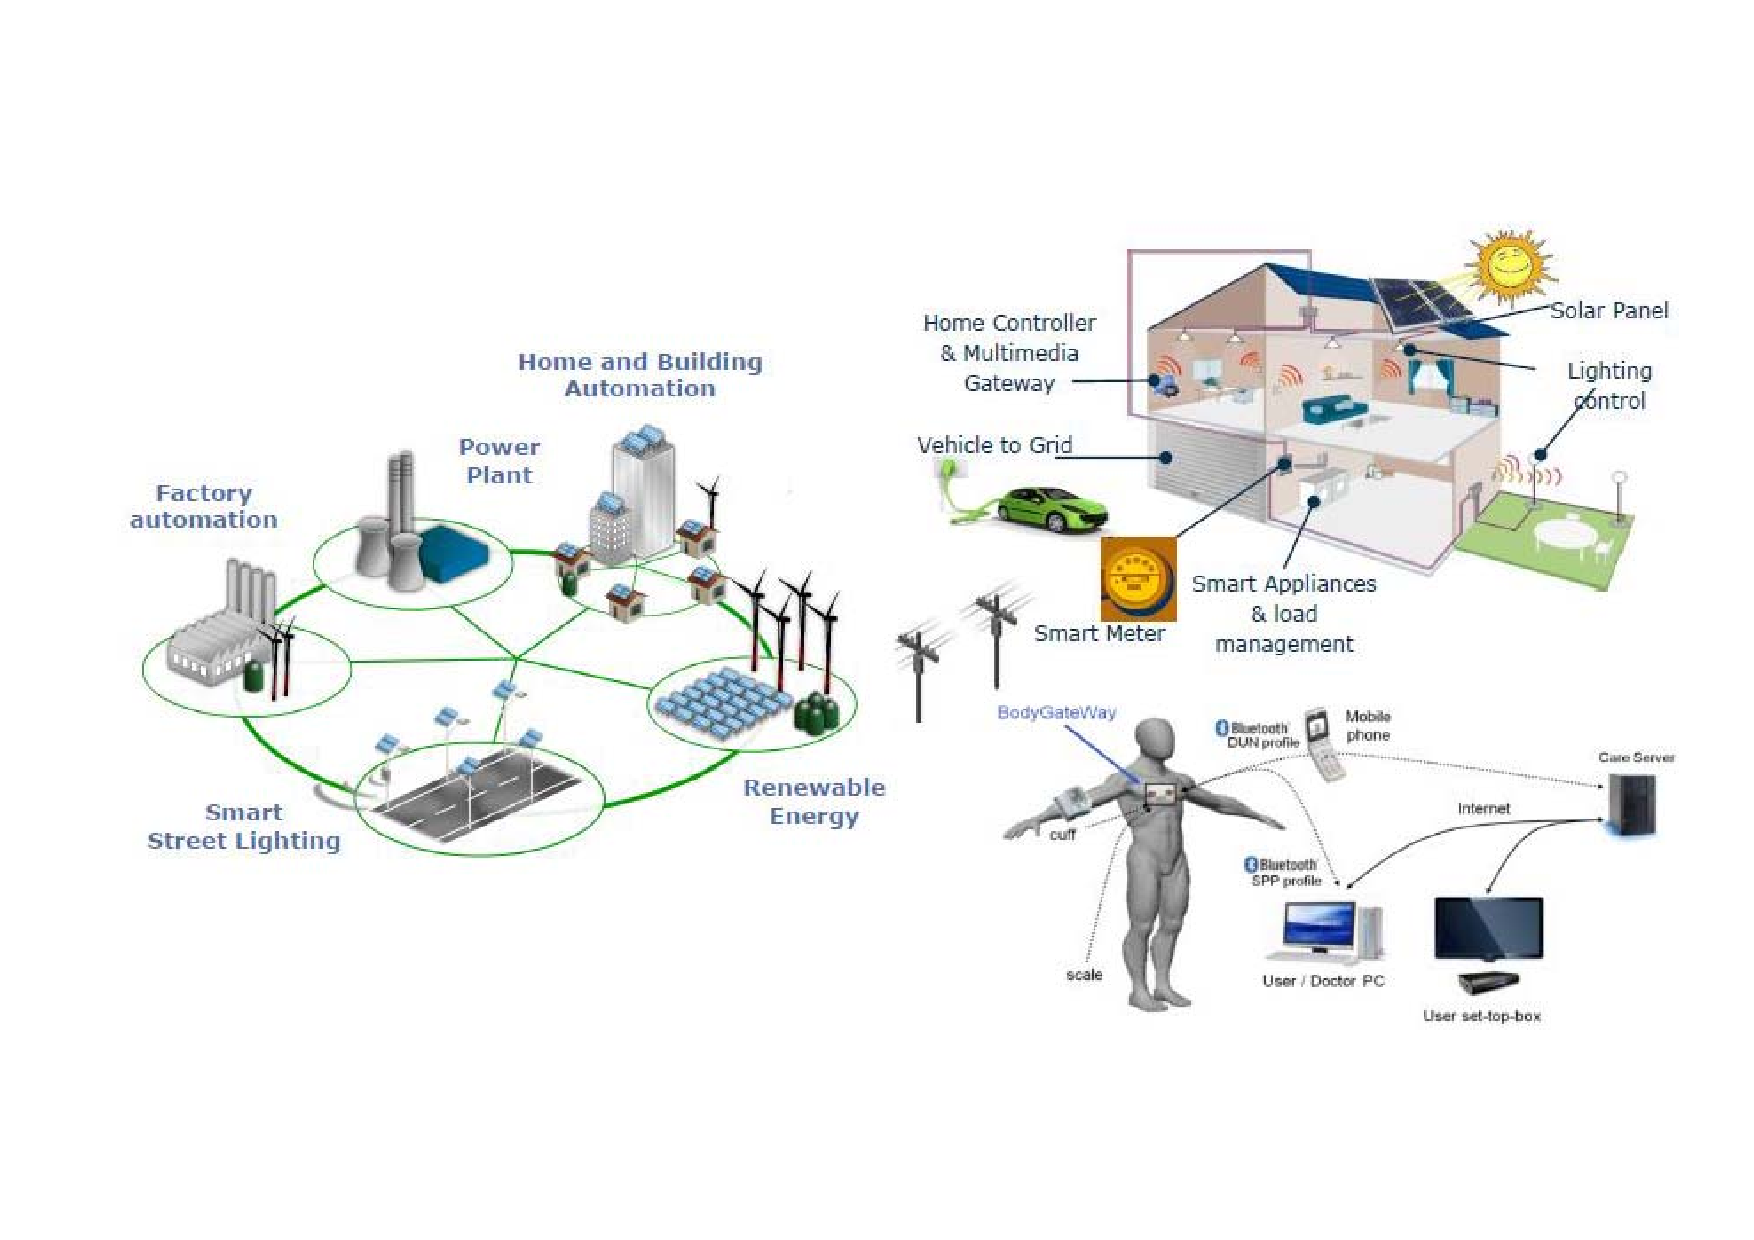
\includegraphics[width=0.55\textwidth]{fig.pdf}
 \vspace{-4mm} 
 \caption{Examples of wireless sensor networks.}
 \vspace{-4mm}
  \label{fig:scenario}
\end{figure}


In this respect, fits the present work.
The remainder of this report is organized as follows. In section
\ref{sec:sa}, we present some related works in a sort of a state of the art
about self configuration of WSNs. This section is subdivided in three parts
describing respectively the concept of self configuration related to the WSNs architecture, the applications and services in these networks, and the systems
and networking in these lasts. Overall evaluations about the works are
discussed in Section~\ref{sec:ev}. Finally, Section~\ref{sec:conclusions} concludes the paper.
